\documentclass{mwart} % Polska wersja klasy article

\usepackage{polski} % Pozwala na użycie polskiego. Ustawia między innymi fontenc na T1
\usepackage[utf8]{inputenc} % Informuje o kodowaniu
\usepackage{textcomp} % Znaki specjalne takie jak ~
\usepackage{xcolor} % Definicje kolorów

\renewcommand{\labelitemi}{\textbullet} % Zmiana symbolu wliczeń

\usepackage{graphicx}
\graphicspath{ {./Obrazy/} }
% \usepackage{subcaption} % Subfigury
\usepackage{float} % Pozycjonowanie figur
\usepackage{mwe} % Tymczasowe grafiki

\usepackage{listings} % Listingi kodu
\lstset{basicstyle=\ttfamily,
  showstringspaces=false,
  commentstyle=\color{gray},
  keywordstyle=\color{blue}
}

\title{Laboratorium sieci komputerowych - c4 \\ Sieci bezprzewodowe}
\author{Krzysztof Dąbrowski gr. 3}
\date{\today}

\begin{document}
\maketitle{}
\tableofcontents{}
%\newpage

\section{Cel zajęć}
Celem laboratorium jest zbadanie lokalnych sieci radiowych oraz podłączenie i konfiguracja interfejsów radiowych na maszynach z systemami Ubuntu i FreeBSD.

\section{Analiza przestrzeni radiowej}
Przy pomocy aplikacji \textit{Wifi Analyzer} przeskanowałem dostępne sieci radiowe oraz pokrycie poszczególnych kanałów.
Wyniki analizy sieci pokazuje rysunek \ref{fig:wifiAnalizer}.

%TODO: Skompilować gdzieś, gdzie subfigure działa
% \begin{figure}[H]
%     \centering
%     \begin{subfigure}[b]{0.49\textwidth}
%         \centering
%         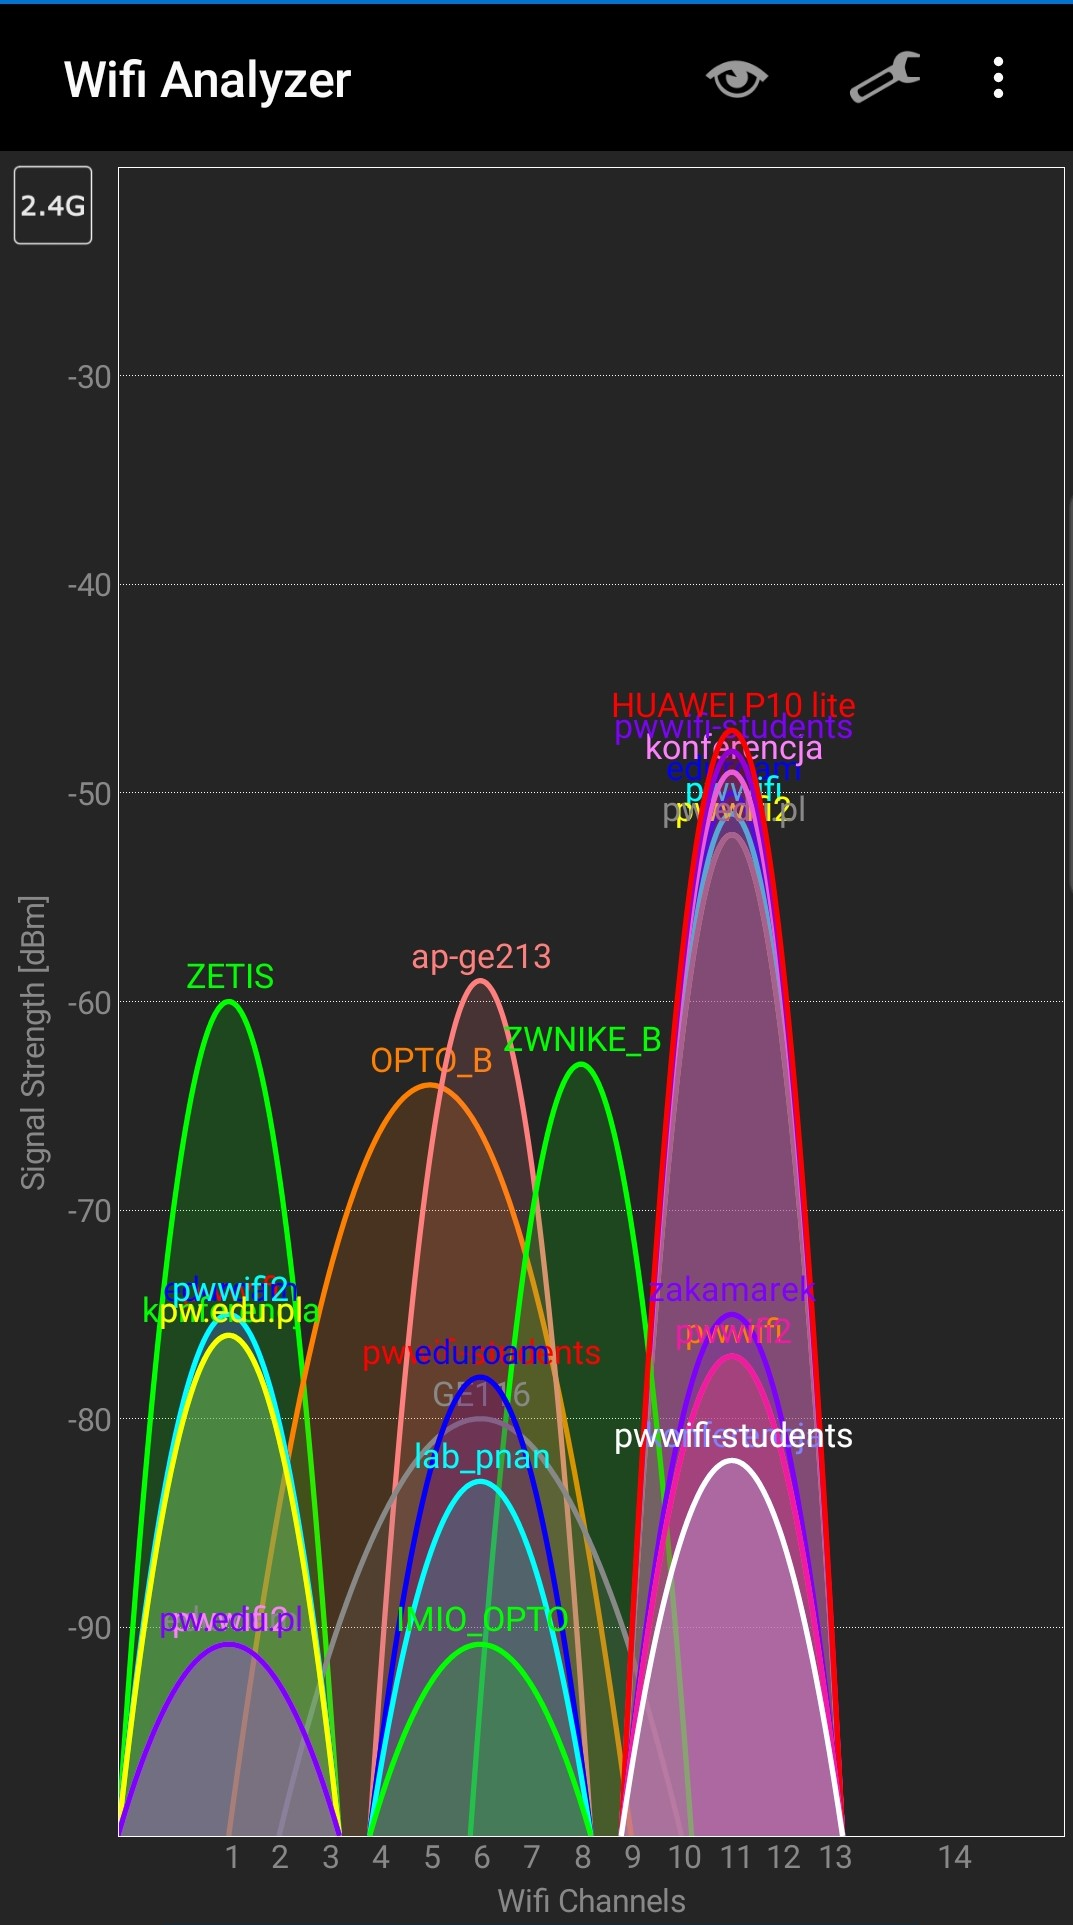
\includegraphics[width=0.4\textwidth]{Sieci-2,4GH}
%         \caption{Sieci na częstotliwości 2,4GHz}
%     \end{subfigure}
%     \begin{subfigure}[b]{0.49\textwidth}
%         \centering
%         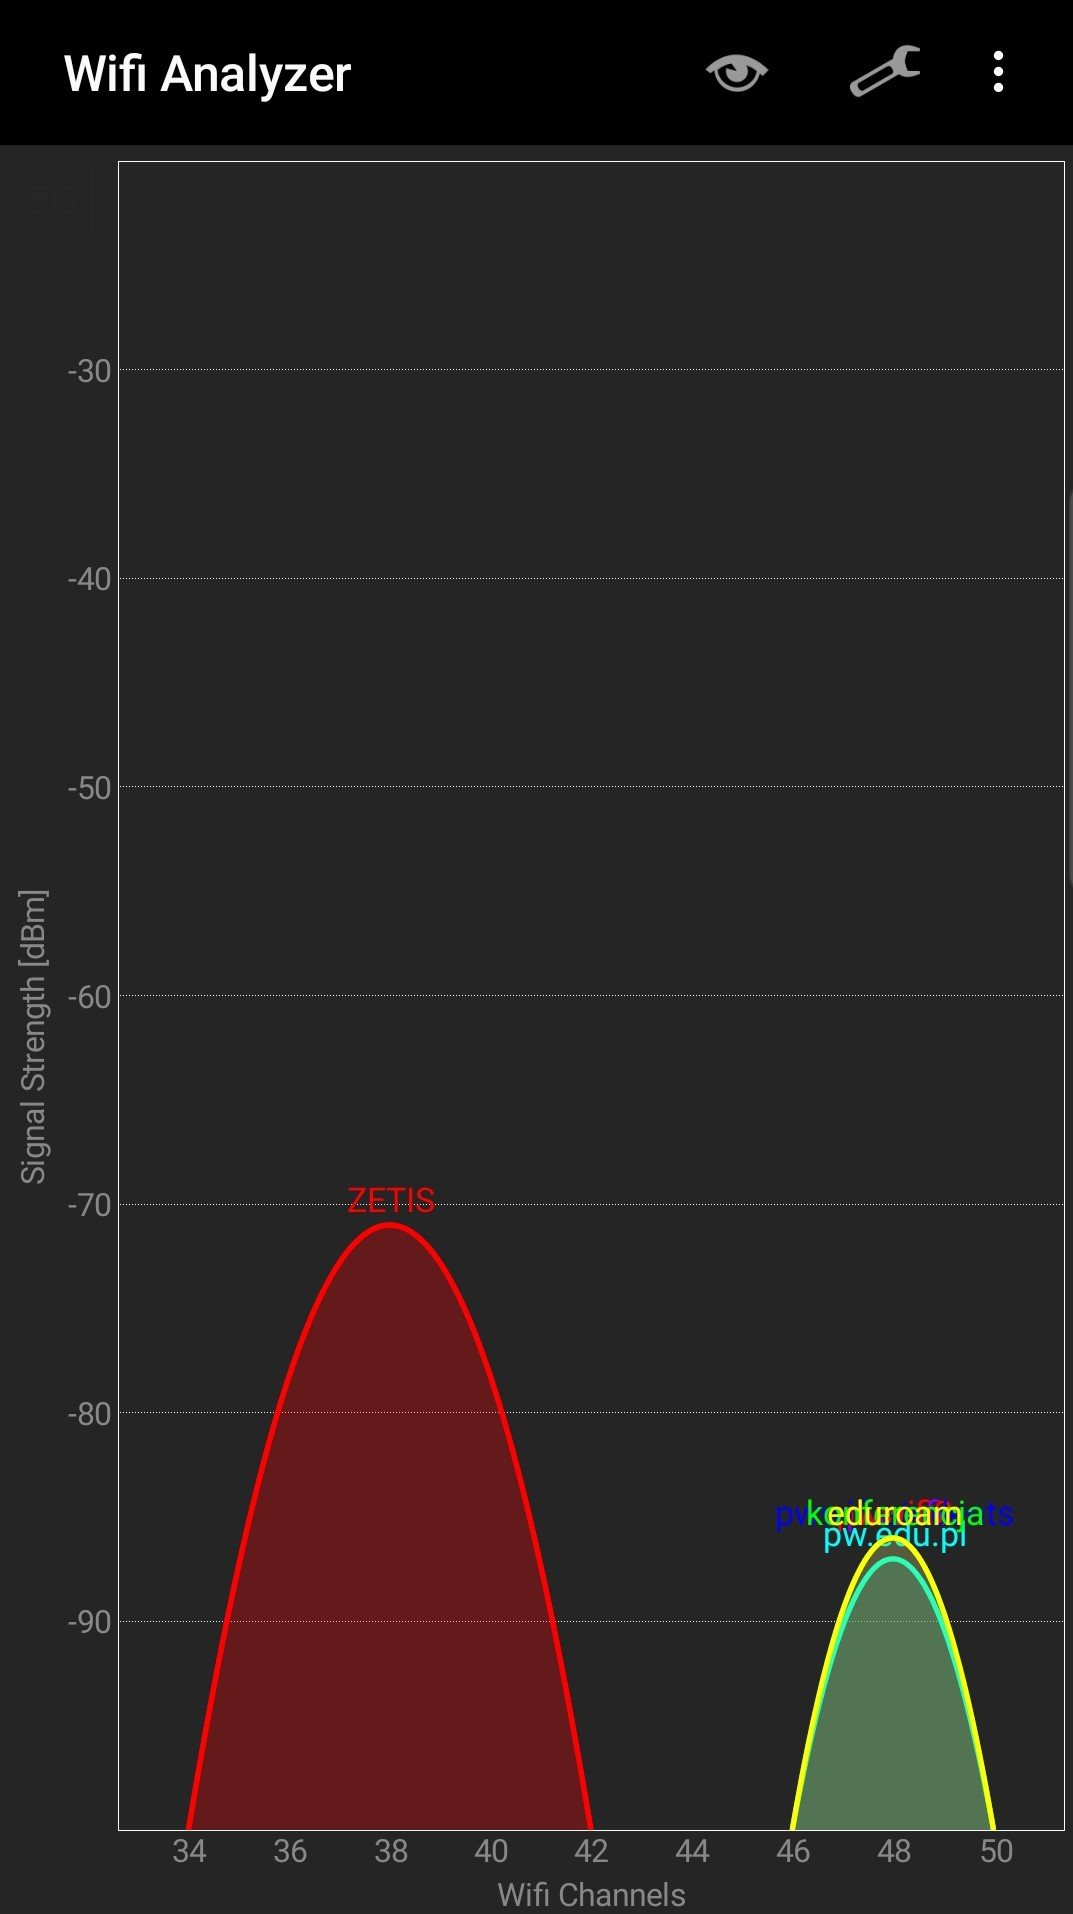
\includegraphics[width=0.4\textwidth]{Sieci-5GH}
%         \caption{Sieci na częstotliwości 5GHz}
%     \end{subfigure}
%     \label{fig:wifiAnalizer}
% \end{figure}

Dodatkowo przeskanowałem dostępne sieci przy pomocy polecenia \texttt{nmcli device wifi list}.

\begin{verbatim}
*  SSID                  MODE   CHAN  RATE    SIGNAL  SECURITY
konferencja           Infra  11    54 Mbit/s  74      WEP
pwwifi-students       Infra  11    54 Mbit/s  30      --
pwwifi2               Infra  11    54 Mbit/s  30      WPA2 802.1X
pwwifi-students       Infra  11    54 Mbit/s  35      --
vlab_net              Infra  11    54 Mbit/s  35      WPA2
konferencja           Infra  11    54 Mbit/s  30      WEP
pwwifi                Infra  11    54 Mbit/s  49      --
ZETIS                 Infra  1     54 Mbit/s  99      WPA2 802.1X
pwwifi-students       Infra  6     54 Mbit/s  34      --
TROL                  Infra  1     54 Mbit/s  29      --
pwwifi2               Infra  1     54 Mbit/s  52      WPA2 802.1X
pwwifi                Infra  11    54 Mbit/s  30      --
pwwifi2               Infra  11    54 Mbit/s  75      WPA2 802.1X
pwwifi2               Infra  6     54 Mbit/s  35      WPA2 802.1X
Sieć Wi-Fi (WE-Lech)  Infra  6     54 Mbit/s  30      WPA2
pwwifi-students       Infra  6     54 Mbit/s  37      --
Stery3                Infra  11    54 Mbit/s  30      WPA1 WPA2
asdf                  Infra  9     54 Mbit/s  49      WPA1 WPA2
pwwifi2               Infra  6     54 Mbit/s  30      WPA2 802.1X
linksys               Infra  3     54 Mbit/s  24      WPA2
konferencja           Infra  1     54 Mbit/s  54      WEP
konferencja           Infra  6     54 Mbit/s  40      WEP
konferencja           Infra  1     54 Mbit/s  37      WEP
konferencja           Infra  6     54 Mbit/s  34      WEP
is_wifi               Infra  4     54 Mbit/s  30      WEP
konferencja           Infra  6     54 Mbit/s  30      WEP
pwwifi                Infra  1     54 Mbit/s  54      --
pwwifi-students       Infra  1     54 Mbit/s  49      --
pwwifi                Infra  6     54 Mbit/s  44      --
pwwifi                Infra  1     54 Mbit/s  37      --
pwwifi-students       Infra  11    54 Mbit/s  30      --
pwwifi2               Infra  1     54 Mbit/s  42      WPA2 802.1X
pwwifi2               Infra  6     54 Mbit/s  32      WPA2 802.1X
konferencja           Infra  1     54 Mbit/s  20      WEP
pwwifi                Infra  1     54 Mbit/s  37      --
pwwifi-students       Infra  1     54 Mbit/s  24      --
pwwifi-students       Infra  1     54 Mbit/s  20      --
\end{verbatim}

\section{Schemat sieci}
Strukturę urządzeń w sieci przedstawia rysunek \ref{fig:SchematSieci}.

\begin{figure}[H]
  \centering
  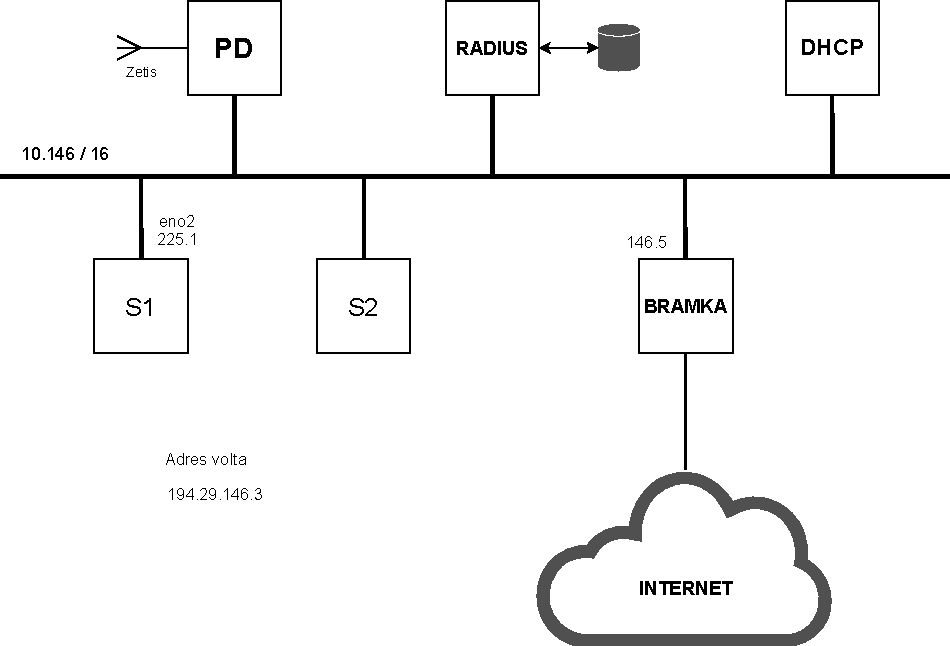
\includegraphics[width=\textwidth]{SchematSieci}
  
  \caption{Schemat sieci}
  \label{fig:SchematSieci}
\end{figure}

\section{Podłączenie do sieci wifi w środowisku graficznym}
W celu przyłączenia do sieci skorzystam z nakładki graficznej na program \textit{NetworkManager} wbudowanej w system Ubuntu.
\vspace{5 mm}

Przed podłączeniem sprawdziłem stan interfejsu radiowego poleceniem \texttt{ip~a}.
\begin{verbatim}
    ip a

    4: wlp2s0: <NO-CARRIER,BROADCAST,MULTICAST,UP> mtu 1500 qdisc mq state DOWN group default qlen 1000
    link/ether 00:24:d7:92:0e:dc brd ff:ff:ff:ff:ff:ff
\end{verbatim}

Oraz tablicę tras, poleceniem \texttt{ip r}.
\begin{verbatim}
    ip r 

    default via 10.146.146.5 dev eno2
    10.146.0.0/16 dev eno2  proto kernel  scope link  src 10.146.225.1
\end{verbatim}

Z otrzymanych wyników wiać, że interfejs radiowy jest \textbf{nieaktywny} a trasa domyślna wiedzie przez interfejs fizyczny.
\vspace{5 mm}

Po podłączeniu do sieci \textbf{ZETIS} wyniki tych poleceń wyglądały następująco:
\begin{verbatim}
    ip a

    4: wlp2s0: <BROADCAST,MULTICAST,UP,LOWER_UP> mtu 1500 qdisc mq
        state UP group default qlen 1000
    link/ether 00:24:d7:7d:ba:8c brd ff:ff:ff:ff:ff:ff
    inet 10.68.17.233/16 brd 10.68.255.255 scope global dynamic wlp2s0
       valid_lft 3601sec preferred_lft 3601sec
    inet6 fe80::224:d7ff:fe7d:ba8c/64 scope link 
       valid_lft forever preferred_lft forever
\end{verbatim}

\begin{verbatim}
    ip r 

    default via 10.146.146.5 dev eno2 
    default via 10.68.0.1 dev wlp2s0  proto static  metric 600 
    10.68.0.0/16 dev wlp2s0  proto kernel  scope link  src 10.68.17.233  metric 600 
    10.146.0.0/16 dev eno2  proto kernel  scope link  src 10.146.225.3 
    169.254.0.0/16 dev wlp2s0  scope link  metric 1000 
    192.0.2.4 via 10.68.0.1 dev wlp2s0  proto dhcp  metric 600 
\end{verbatim}

Widać, że interfejs radiowy \texttt{wlp2s0} jest teraz włączony oraz skonfigurowany.
Do tablicy tras została dodana nowa domyślna trasa prowadząca przez interfejs radiowy.
\vspace{5 mm}

Dodatkowo pobrałem logi z serwera RADIUS połączeniem komend \texttt{ssh ldap grep -w \$USER /var/log/radiusd | tail -2}.
\begin{verbatim}
    ssh ldap grep -w \$USER /var/log/radiusd | tail -2

    Mon May 13 17:01:43 2019 : Auth: (2156)   Login OK: [dabrowk1] 
        (from client ap225 port 0 via TLS tunnel)
    Mon May 13 17:01:43 2019 : Auth: (2156) Login OK: [dabrowk1]
        (from client ap225 port 0 cli 00-22-3F-01-F9-12)
\end{verbatim}
Z zebranych logów wynika, że serwer RADIUS zaakceptował podane dane dostępowe.

Po podłączeniu do sieci \textbf{pw.edu.pl} stan interfejsów i tras wyglądał następująco:

\begin{verbatim}
    ip a

    5: wlx00223f01f912: <BROADCAST,MULTICAST,UP,LOWER_UP> mtu 1500 qdisc mq
        state UP group default qlen 1000
    link/ether 00:22:3f:01:f9:12 brd ff:ff:ff:ff:ff:ff
    inet 10.68.31.177/16 brd 10.68.255.255 scope global dynamic wlx00223f01f912
       valid_lft 3387sec preferred_lft 3387sec
    inet6 fe80::222:3fff:fe01:f912/64 scope link 
       valid_lft forever preferred_lft forever
\end{verbatim}

\footnotesize{}
\begin{verbatim}
    netstat -nr

    Destination     Gateway         Genmask         Flags   MSS Window  irtt Iface
    0.0.0.0         10.146.146.5    0.0.0.0         UG        0 0          0 eno1
    0.0.0.0         10.68.0.1       0.0.0.0         UG        0 0          0 wlx00223f01f912
    10.68.0.0       0.0.0.0         255.255.0.0     U         0 0          0 wlx00223f01f912
    10.146.0.0      0.0.0.0         255.255.0.0     U         0 0          0 eno1
    169.254.0.0     0.0.0.0         255.255.0.0     U         0 0          0 wlx00223f01f912
    192.0.2.4       10.68.0.1       255.255.255.255 UGH       0 0          0 wlx00223f01f912
\end{verbatim}
\normalsize{}

\section{Podłączenie w środowisku tekstowym na Ubuntu}
Domyślnie konfiguracją interfejsów radiowych zarządza program \textit{NetworkManager}. Musiałem go wyłączyć by dokonać ręcznej konfiguracji.

Wyłączyłem ten program przy pomocy poleceń \texttt{sudo systemctl stop NetworkManager.service} oraz \texttt{sudo systemctl disable NetworkManager.service}.

Aby sprawdzić czy serwis został wyłączony wywołałem \texttt{sudo systemctl status NetworkManager.service}.
\begin{verbatim}
    sudo systemctl status NetworkManager.service

    * NetworkManager.service - Network Manager
   Loaded: loaded (/lib/systemd/system/NetworkManager.service; disabled; vendor
   Active: inactive (dead) since pon 2019-05-13 17:51:50 CEST
    Main PID: 1458 (code=exited, status=0/SUCCESS)
\end{verbatim}
\vspace{5 mm}

Do połączenia się z siecią ZETIS skorzystam z programu \texttt{wpa\_supplicant}.

Plik konfiguracyjny wygenerowałem poleceniem \texttt{wpa-config-zetis}. Ma on następującą treść:
\begin{verbatim}
    trl_interface=/var/run/wpa_supplicant  # dla wpa_cli

    eapol_version=1
    ap_scan=1

    network={
    priority=30
    ssid="ZETIS"
    proto=WPA2
    key_mgmt=WPA-EAP  identity="dabrowk1"   # login
    password=hash:73a1da770586527f5d97f02a136a7795        # haslo 
}
\end{verbatim}
Wygenerowany plik zapisałem w katalogu \texttt{/etc/wpa\_supplicant/wpa\_supplicant.conf}.

\vspace{5 mm}
Uruchomiłem demona wpa\_supplicant poleceniem \\\texttt{sudo wpa\_supplicant -B -i wlp2s0 -c /etc/wpa\_supplicant/wpa\_supplicant.conf}.
Po wykonaniu tego polecenia system wyświetlił komunikat \texttt{Successfully initialized wpa\_supplicant}.

\paragraph{Stan interfejsu radiowego} po wykonaniu tych czynności uległ zmianie.
\begin{verbatim}
    ip a

    4: wlp2s0: <BROADCAST,MULTICAST,UP,LOWER_UP> mtu 1500 qdisc mq state UP group default qlen 1000
    link/ether 00:24:d7:92:0e:dc brd ff:ff:ff:ff:ff:ff
\end{verbatim}
Widać, że jest teraz włączony.

\paragraph{Pobranie adresu ip} na interfejsie radiowym wykonałem poleceniem \texttt{sudo dhclient wlp2s0}. Oraz sprawdziłem otrzymany adres poleceniem \texttt{ip}.
\begin{verbatim}
    ip a

    4: wlp2s0: <BROADCAST,MULTICAST,UP,LOWER_UP> mtu 1500 qdisc mq state UP group default qlen 1000
    link/ether 00:24:d7:92:0e:dc brd ff:ff:ff:ff:ff:ff
    inet 10.146.90.130/16 brd 10.146.255.255 scope global wlp2s0
       valid_lft forever preferred_lft forever
\end{verbatim}

\paragraph{Dziennik RADIUS} został zaktualizowany o wpis dotyczący tego połączenia.
Przeczytałem jego zawartość poleceniem \texttt{ssh ldap grep -w \$USER /var/log/radiusd | tail -2}
\begin{verbatim}
    ssh ldap grep -w $USER /var/log/radiusd | tail -2

    Mon May 20 21:57:20 2019 : Auth: (1401)   Login OK: [dabrowk1] 
        (from client ap225 port 0 via TLS tunnel) 
    Mon May 20 21:57:20 2019 : Auth: (1402) Login OK: [dabrowk1] 
        (from client ap225 port 0 cli 00-24-D7-92-0E-DC)
\end{verbatim}

\paragraph{Dziennik DHCP} również posiada wpis opisujący przydzielenie adresu.
\begin{verbatim}
    cat /var/log/syslog | grep -Ei 'dhcp' | tail -3

    May 20 20:03:33 s1 dhclient[8615]: DHCPOFFER of 10.146.90.130 from 10.146.146.25 
    May 20 20:03:33 s1 dhclient[8615]: DHCPACK of 10.146.90.130 from 10.146.146.25
    May 20 20:03:33 s1 dabrowk1: /etc/dhcp/dhclient-enter-hooks.d/avahi-autoipd returned non-zero exit status 1
\end{verbatim}

Mogę przeczytać szczegóły przydzielonych dynamicznie wartości poleceniem \texttt{cat /var/lib/dhcp/dhclient.leases}.

\subsection*{Zmiana domyślnej trasy}
W celu przekierowania ruchu przez interfejs radiowy zmieniłem trasę domyślną.

Usunąłem trasę domyślną przez interfejs \texttt{eno2} poleceniem \texttt{sudo ip route delete default} oraz ustawiłem nową poleceniem \texttt{sudo ip route add default via 10.146.146.5 dev wlp2s0}.
\vspace{2mm}

Stan tablicy tras po zmianie:
\begin{verbatim}
    ip r

    default via 10.146.146.5 dev wlp2s0  
    10.146.0.0/16 dev eno2  proto kernel  scope link  src 10.146.225.1
    10.146.0.0/16 dev wlp2s0  proto kernel  scope link  src 10.146.90.130
\end{verbatim}

\subsection*{Sprawdzenie trasy pakietów}
By zweryfikować czy ustawiona trasa działa poprawnie skorzystałem z poleceń \texttt{traceroute} i \texttt{ping}.

\begin{verbatim}
    traceroute  volt

    1  * * * 
    2  volt.iem.pw.edu.pl (194.29.146.3)  6.531 ms  6.535 ms  6.539 ms
\end{verbatim}
Widać, że trasa wygląda inaczej niż gdy połączenie było przez interfejs eno2.

\begin{verbatim}
    ping -c 1 google.com

    PING google.com (172.217.16.14) 56(84) bytes of data. 
    64 bytes from mil02s06-in-f14.1e100.net (172.217.16.14): icmp_seq=1 ttl=54 time=114 ms 
\end{verbatim}
Po wyniku pinga widać większe opóźnienie (114 ms) co jest charakterystyczne dla sieci radiowych.

\section{Podłączenie w środowisku tekstowym na FreeBSD}
By przygotować stację do pracy zalogowałem się jako \texttt{root} zamontowałem katalog publiczny oraz uruchomiłem skrypt \texttt{labsk}




Zrobiłem to poleceniami \texttt{mount /pub} oraz \texttt{/pub/FreeBSD/zetis/config/labsk}.

Po ponownym zalogowaniu na stację była ona gotowa do pracy.

\end{document}